%---------------------------4.1-----------------------------------%
\section{Experiments Platform}

%-------------------------4.1.1----------------------------------%
\subsection{Experiments Design}
\label{Experiments_design_subsection}

Icart-mini \cite{icart_mini} and VLP-16 LiDAR \cite{vlp16} are the robot and sensor used in this investigation. 
A laptop will be mounted on the robot, it connects to the LiDAR, does 
processing and calculations, and issues orders to the robot. Icart-mini is a 
T-frog robot that has a simple design and can be moved both indoors and outdoors. 
This robot template is available for free. The supplier has offered a variety of 
packages to help users create apps for Icart-mini. Being the smallest in the Velodyne 
product range, the VLP-16 LiDAR scanner, was developed at a low cost with mass 
production in mind, notably for robots, autonomous cars, and industrial automation.

\begin{figure}[h]
    \centering
    \begin{subfigure}{.5\linewidth}
        \centering
        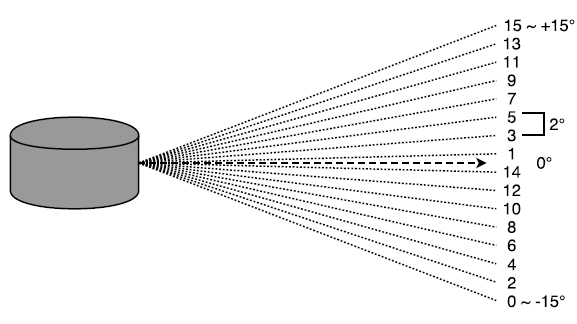
\includegraphics[width=1.0\linewidth,height = 0.5\linewidth]{figures/chap4_fig/Platform/lidar_property.png}
          \caption{LiDAR property \cite{lidarproperties}}
        \label{chap4:fig1:sub1}
    \end{subfigure}%
    \begin{subfigure}{.5\linewidth}
        \centering
        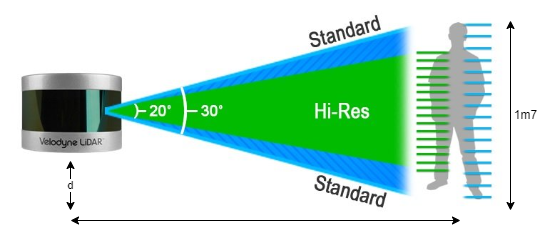
\includegraphics[width=1.0\linewidth,height = 0.5\linewidth]{figures/chap4_fig/Platform/Untitled Diagram-Page-12.drawio.png}
          \caption{Model calculate height of LiDAR \cite{calculateheight}}
        \label{chap4:fig1:sub2}
    \end{subfigure}
    \caption{VLP-16 LiDAR vertical field of view}
    \label{chap4:fig1}
\end{figure}


\begin{table}[h!]
    \centering
    \begin{tabular}{||c|c||}
        \hline
        \rowcolor{lightgray}
        \textbf{Item}                 & \textbf{Specifications}                     \\ [0.5ex]
        \hline\hline
        Scanning rate                 & 10 scans/s                                  \\ \hline
        Horizontal field of view      & $360^o$                                     \\ \hline
        Horizontal angular resolution & $0.23^o$                                    \\ \hline
        Vertical field of view        & $26.8^o$                                    \\ \hline
        Vertical angular resolution   & $2^o$ (16 lines)                            \\ \hline
        Detection range               & 40m for pavement, 120m for cars and foliage \\ \hline
        Range accuracy                & 0.02m                                       \\ \hline
        Wavelength of laser beam      & 905nm                                       \\ [0.5ex]
        \hline
    \end{tabular}
    \caption{3D VLP-16 LiDAR properties \cite{vlp16}}
    \label{Chap4:Table1}
\end{table}


\begin{figure}[!htb]
    \centering
    % \hspace*{-8mm}
    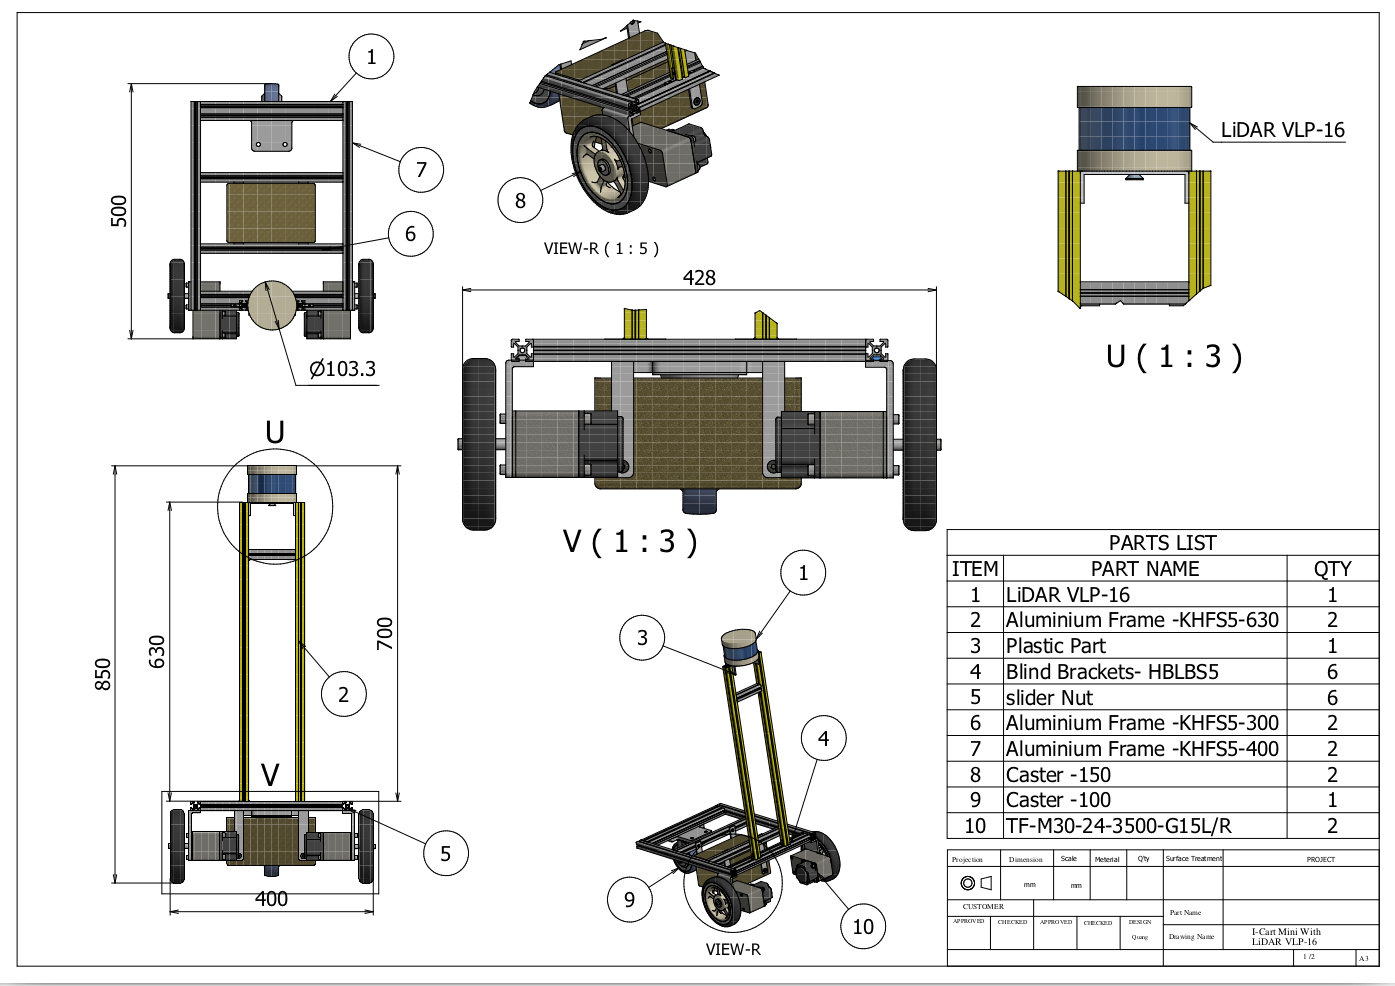
\includegraphics[width=1.0\linewidth]{figures/chap4_fig/Platform/Icart_mini_withLidar_drawing.png}
    \caption{Design of VLP-16 LiDAR onboard Icart-mini robot}
    \label{chap4:fig2}
\end{figure}



\begin{figure}[h]
    \centering
    % \hspace*{-8mm}
    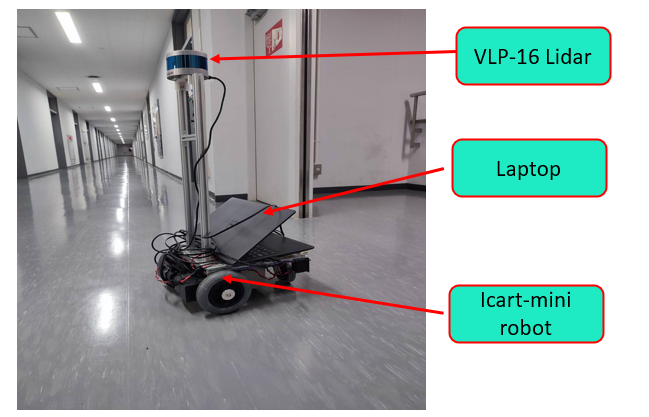
\includegraphics[width=1.0\linewidth]{figures/chap4_fig/Platform/icart_mini_with_lidar.png}
    \caption{Final experiments design in real life}
    \label{Chap4:fig3}
\end{figure}

Figure \ref{chap4:fig1:sub1} and Table \ref{Chap4:Table1}  show the scan properties of 
VLP-16. From these data, one knows that VLP-16 has a total of 16 scans. Each scanning 
ray is aligned at an angle of 2 degrees. The total vertical field of view is 30 degrees. 
The scan range that is considered to be the most detailed will have a scan range of 20 
degrees and a standard of 30 degrees. Consequently, in order to obtain the most complete 
and accurate information about people, we need to place the LiDAR at a certain distance 
from the ground. The height calculation model is shown as Figure \ref{chap4:fig1:sub2} 
below. Assume the minimum distance for the robot to recognize people is at least 2m from 
the robot. The average height of a person is 170cm. From the model, we can calculate 
that the height of the LiDAR will be approximately 80cm from the ground. 
After calculating the required height for the LiDAR, we proceed to fabricate and 
assemble the necessary parts to mount the LiDAR on the robot. The robot model equipped 
with LiDAR is shown in Figure \ref{chap4:fig2}. We used aluminum rods buying from \textit{Misumi}
to connect Icart-mini and VLP-16. The height from the ground to the top of the LiDAR is 
85cm. Figure \ref{Chap4:fig3} displays the full robot model with all of its components. 
A laptop with Ubuntu Operating System will be the processor of the robot. 
In other words, this laptop will be put on top of Icart-mini and acts as the mind of 
the robot. In this laptop, ROS Noetic 20.04 was installed to run the pipeline.


%-------------------------4.1.2----------------------------------%
\subsection{Experiments Setup and Simulations}

In this study, we experimented with the system of robot following people in three 
environments: simulation (Gazebo environment), corridor and hall environment. 
To greatly increase comparability, and make the research project reusable for other
researchers, which indicate that the experiment can be completely recreated without
the necessity to rearrange the real life experiment, we decided to build all
models in Gazebo simulated environment .With the Gazebo environment, it is used to train 
the model, test the PID algorithm and the tracking algorithm.

\begin{figure}[!htb]
    \centering
    % \hspace*{-8mm}
    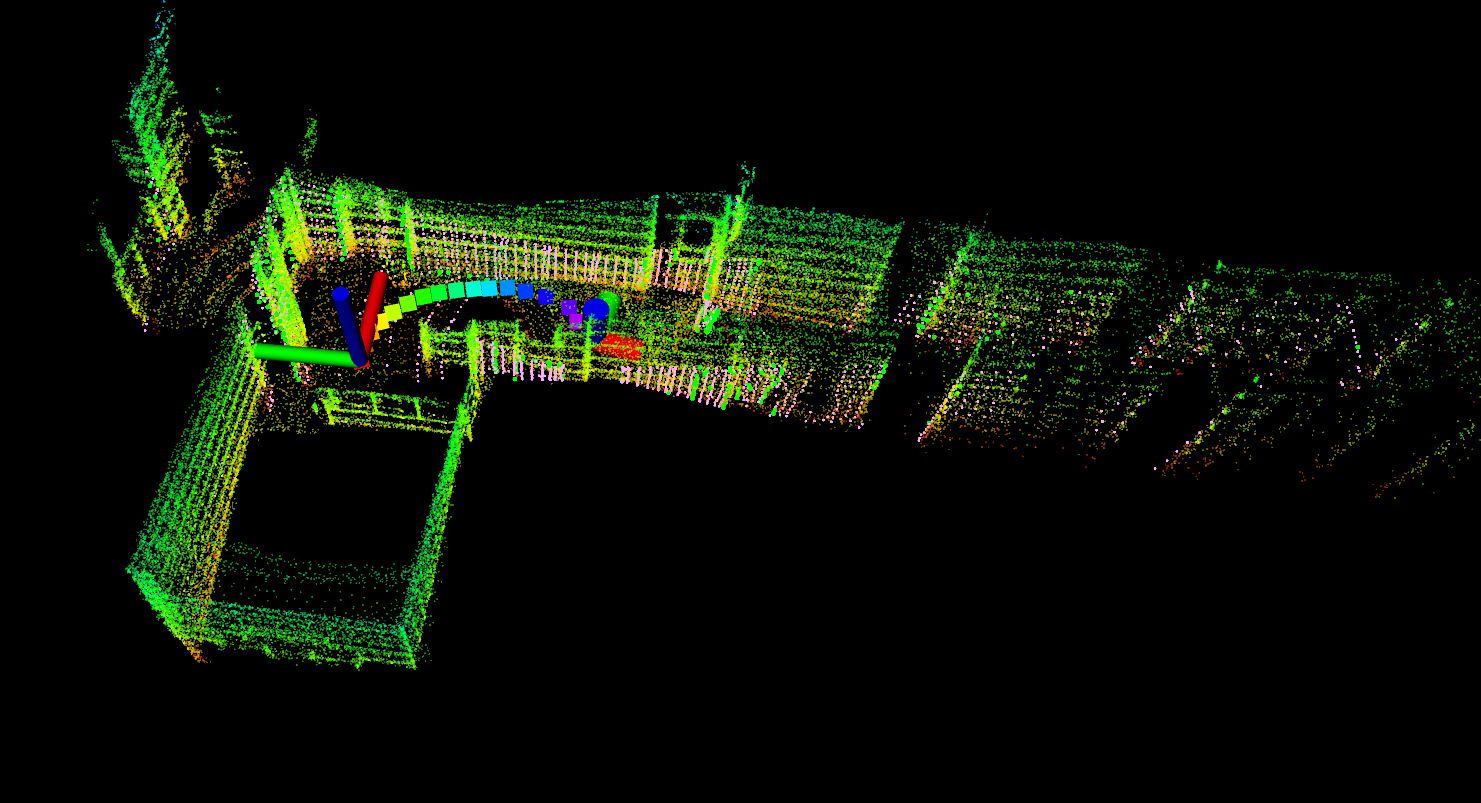
\includegraphics[scale=0.26]{figures/chap4_fig/Platform/Lego-loam-map.png}
    \caption{Corridor 3D Map}
    \label{Chap4:Fig12}
\end{figure}

\begin{figure}[!htb]
    \centering
    % \hspace*{-8mm}
    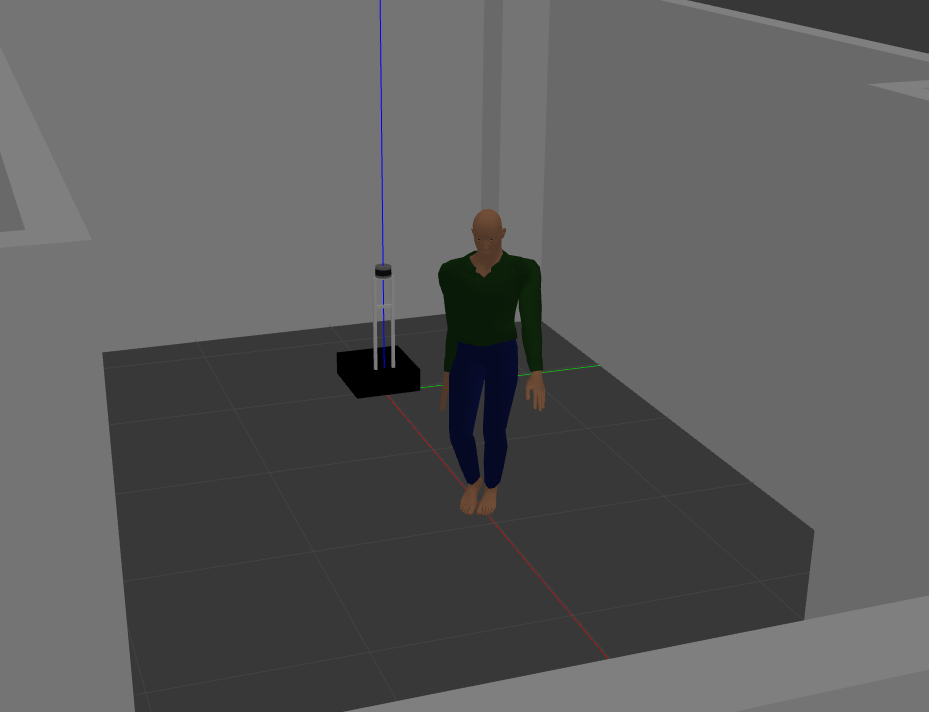
\includegraphics[scale=0.3]{figures/chap4_fig/Platform/human_simulation.png}
    \caption{Human walking simulation using waypoint generator}
    \label{Chap4:Fig11}
\end{figure}

First, for the Gazebo simulation environment, we created an environment 
that was structured like a hallway, which we later used for experiments. In order to 
create the corridor environment as close to reality, we use the ALOAM algorithm 
\cite{legoloam,loam} to scan the corridor area map as illustrated in Figure \ref{Chap4:Fig12}. As we showed in the previous 
workshop, ALOAM is a fairly accurate map scanning algorithm and gives fast results. 
After creating the corridor map, we extracted the images of the map and imported them 
into Gazebo software to create the environment in 1:1 size. In addition, we also added a 
human object environment to train the robot as well as test the algorithm. 
This object will be defined with a certain and repetitive motion trajectory in the environment.
Simulated walking human using waypoint generator is indicated in Figure \ref{Chap4:Fig11}.

\begin{figure}[!htb]
    \begin{subfigure}{.5\linewidth}
        \centering
        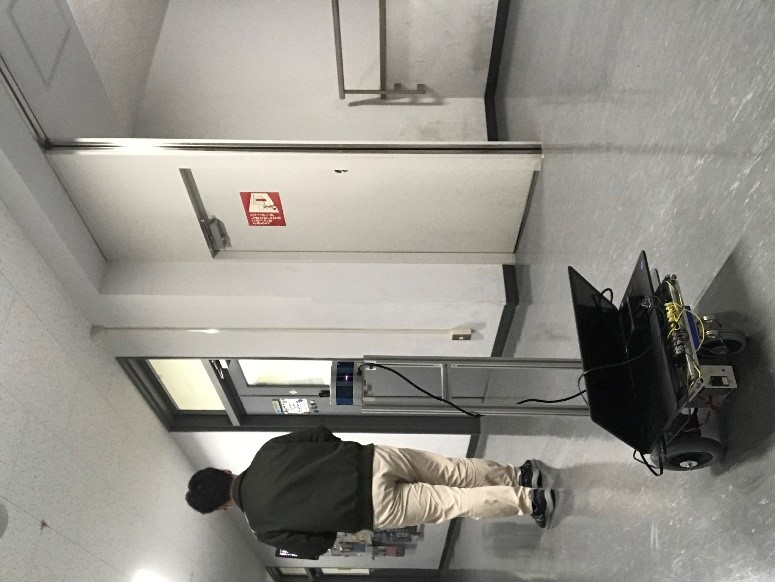
\includegraphics[scale=0.34,angle = -90]{figures/chap4_fig/Platform/corridor_env.jpg}
        \caption{Corridor environment}
        \label{chap4:fig4:sub1}
    \end{subfigure}%
    \begin{subfigure}{.5\linewidth}
        \centering
        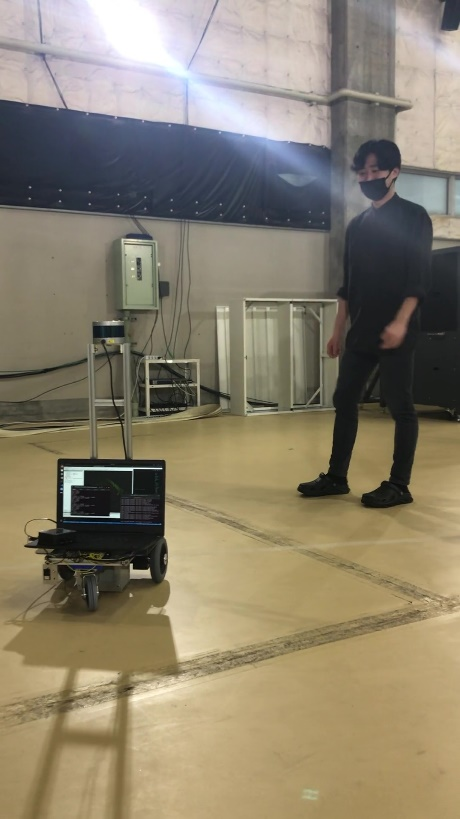
\includegraphics{figures/chap4_fig/Platform/hall_environment.jpg}
        \caption{Testing hall environment}
        \label{chap4:fig4:sub2}
    \end{subfigure}\\[1ex]
    \begin{subfigure}{\linewidth}
        \centering
        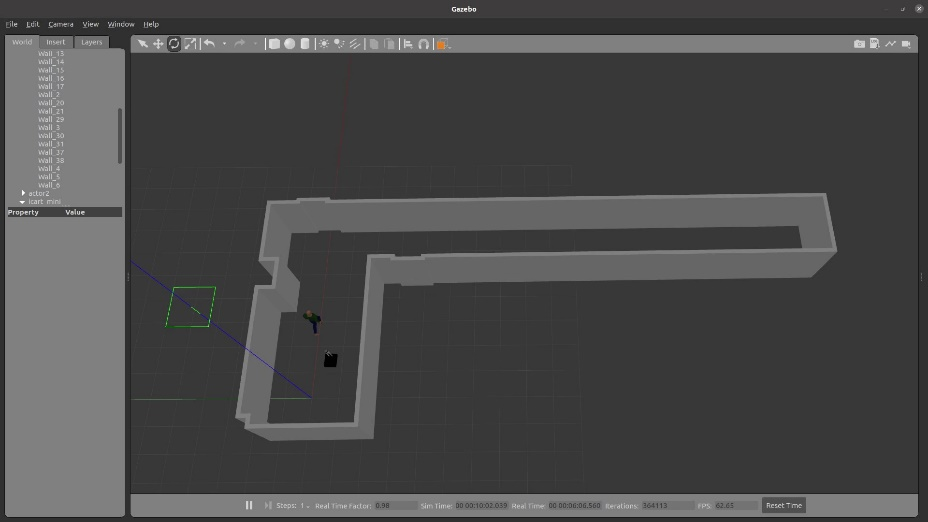
\includegraphics{figures/chap4_fig/Platform/gazebo_environment.jpg}
        \caption{Gazebo environment}
        \label{chap4:fig4:sub3}
        \end{subfigure}
    \caption{Experiment setup in 3 cases}
    \label{Chap4:fig4}
\end{figure}


For experiments conducted in the real environment which includes
the corridor and the aerospace testing hall, robot as in Figure \ref{Chap4:fig3} is 
placed with one participant such as the author himself or author's
friend from laboratory. All experiments are illustrated in Figure \ref{Chap4:fig4}. 
More specifically, Figure \ref{chap4:fig4:sub1} shows the experiment in the corridor, Figure
\ref{chap4:fig4:sub2} shows the experiment in the aerospace testing hall and Figure 
\ref{chap4:fig4:sub3} shows the experiment in the simulated Gazebo environment respectively.

% \newpage
\clearpage

%---------------------------4.2-----------------------------------%
\section{Experiments Results}
\label{Exp_result}

%-----------------------4.2.1-----------------------------%
\subsection{Clustering result}
\label{cluster_result}

This section shows the outcome of point cloud clustering whose method was described in section \ref{Euclidean_cluster_section}.
There are more objects in the aerospace testing hall than in the corridor so the efficiency of the Adaptive clustering technique
is evident in the case of hall environment. For point cloud sets of the same size as a standard human,
we can observe that they are clustered flawlessly without any errors whereas bigger objects in the hall (Figure \ref{Chap3:Fig11})
are sometimes being divided into smaller objects. This is reasonable because their dimensions
belong to various LiDAR's horizontal detected range. Walls in the corridor also behave in the similar 
way, as shown in Figure \ref{Chap3:Fig13}. 

\begin{figure}[h]
    \centering
    % \hspace*{-8mm}
    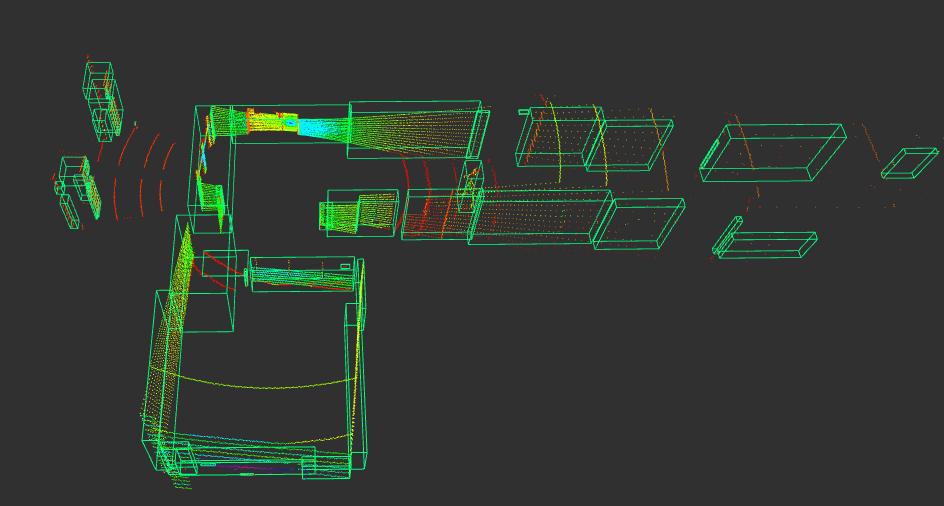
\includegraphics[width=1.0\linewidth]{figures/chap3_fig/euclidean/3_2_7.png}
    \caption{Corridor clustering result}
    \label{Chap3:Fig13}
\end{figure}

\begin{figure}[h]
    \centering
    % \hspace*{-8mm}
    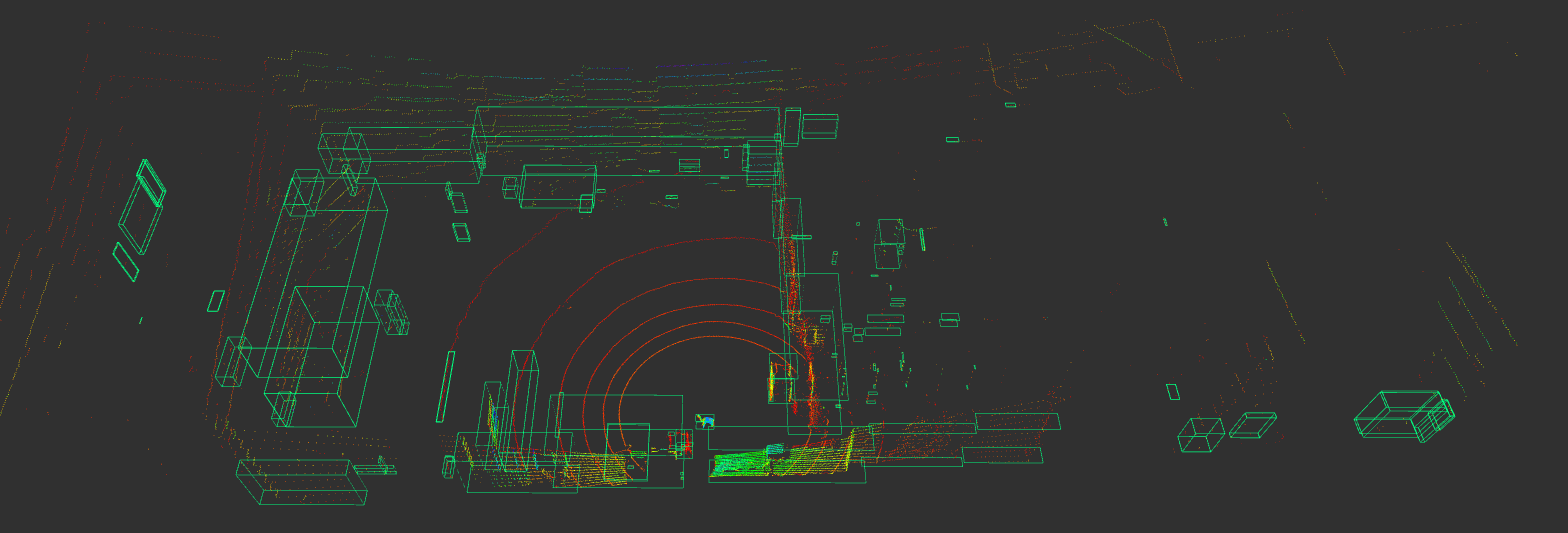
\includegraphics[width=1.0\linewidth]{figures/chap3_fig/euclidean/3_2_5.png}
    \caption{Testing hall clustering result}
    \label{Chap3:Fig11}
\end{figure}

Some objects which are outside the window and not inside the 
corridor are even clustered because of the wide detection range of VLP-16 LiDAR. Those objects are split into multiple smaller 
clusters because they are too far away from the sensor,however, it is not a main issue of the clustering method. This is because 
in this research the distance between human and robot is constrained to be not larger than a maximum value (see section \ref{pid_section}) to 
ensure that human is always clustered into only one cluster and also the inaccuracy of the classification will reduce greatly. Hence, as long as 
human is clustered correctly, this cluster will be treated as positive samples for the next onlin training step. To sum up ,it is appropriate to assert that 
the performance of the adaptive Euclidean clustering in this HFR experiment is acceptable.

% \clearpage



%-----------------------4.2.2-----------------------------%
\subsection{Online training for SVM result}
\label{online_svm_result}

This section displays the consequence of online training whose method was detailed in 
section \ref{online_learning_section}. This training can either be done in two ways: by directly training with robots or by 
recording point cloud into \textit{bag} file and then train later. Both ways will still generate the same result as in 
Figure \ref{Chap4:Fig23}. The result of the online training result can be analysed as follows. First, the SVM human classifier is trained
with a small initial training dataset and shows a poor classification result as in Figure
\ref{Chap4:Fig23:sub1}. After that, the P-N generator will correct wrong samples as described in section 
\ref{online_learning_section} and retrain the whole classifier for better classification result. Then in round 3, we 
can observe from Figure \ref{Chap4:Fig23:sub2} that now there are only 2 clusters are being classified incorrectly as human. When the 
final training round (round 5) is reached, there are no more mis-classified clusters and human cluster is correctly classified, as indicated 
in Figure \ref{Chap4:Fig23:sub3}.

\begin{figure}[!htb]
    \begin{subfigure}{1\linewidth}
        \centering
        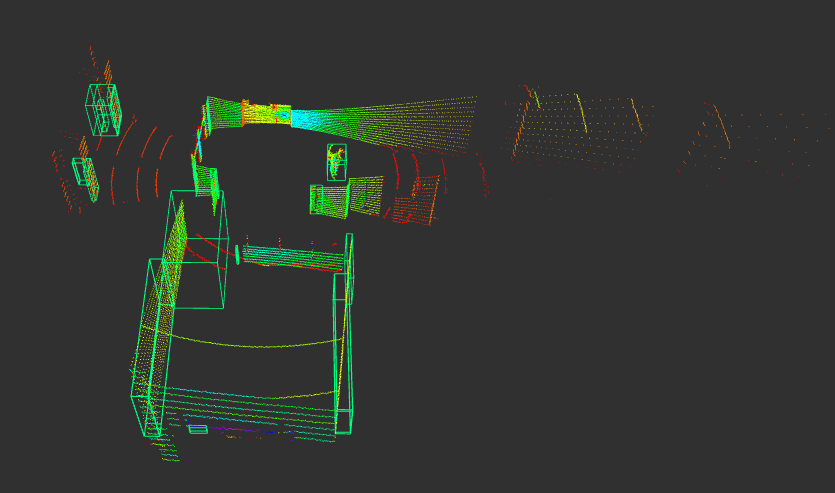
\includegraphics[scale=0.3]{figures/chap3_fig/onlineSVM/online_train_round1.png}
        \caption{Online train round 1 (initial)}
        \label{Chap4:Fig23:sub1}
    \end{subfigure}
    \begin{subfigure}{1\linewidth}
        \centering
        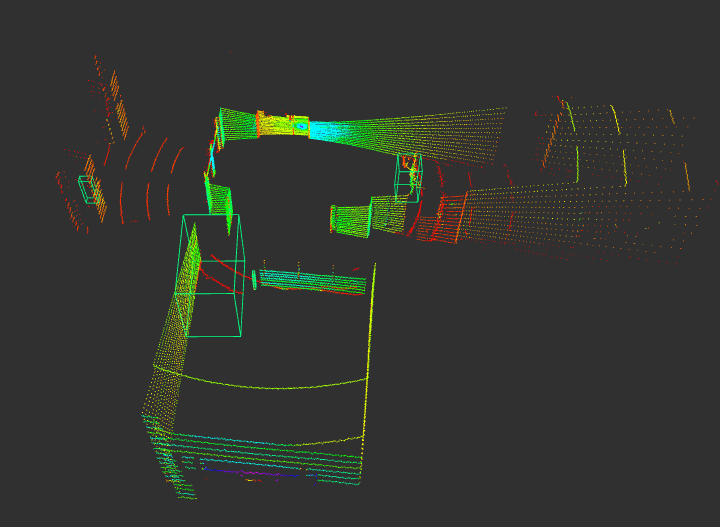
\includegraphics[scale=0.348]{figures/chap3_fig/onlineSVM/online_train_round3.png}
        \caption{Online train round 3}
        \label{Chap4:Fig23:sub2}
    \end{subfigure}
    \begin{subfigure}{1\linewidth}
        \centering
        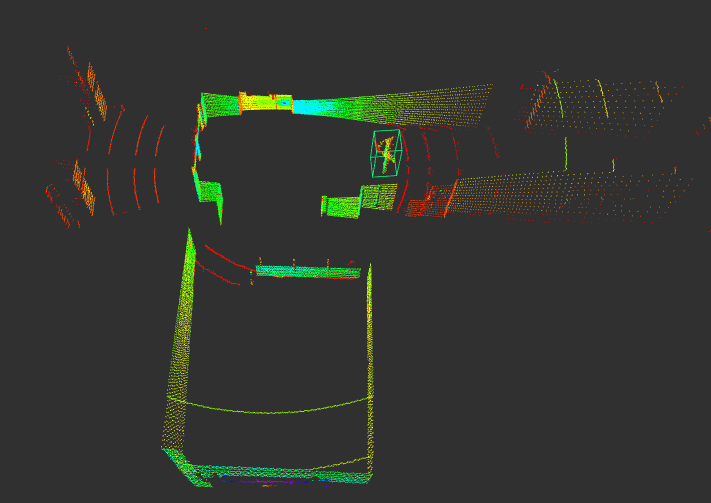
\includegraphics[scale=0.35]{figures/chap3_fig/onlineSVM/online_train_round5.png}
        \caption{Online train round 5}
        \label{Chap4:Fig23:sub3}
    \end{subfigure}
    \caption{Online training result in corridor environment}
    \label{Chap4:Fig23}
\end{figure}

% \begin{figure}[h]
%     \centering
%     % \hspace*{-8mm}
%     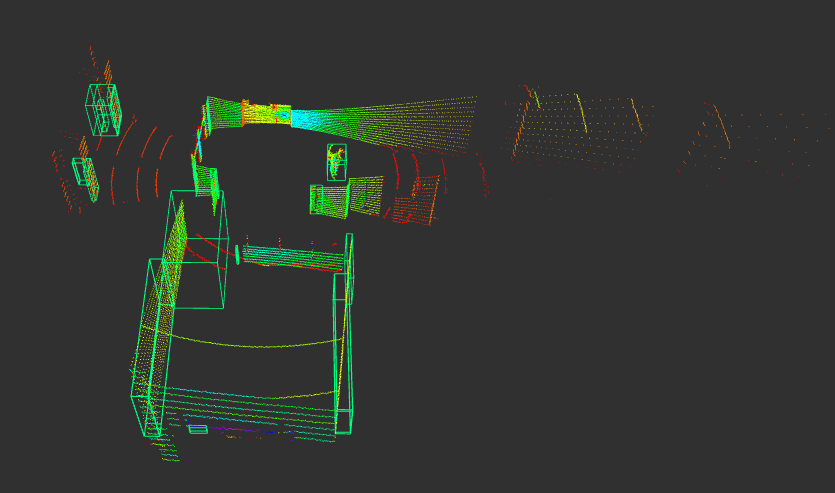
\includegraphics[scale=0.5]{figures/chap3_fig/onlineSVM/online_train_round1.png}
%     \caption{Online train round 1 (initial)}
%     \label{Chap3:Fig17}
% \end{figure}

% \begin{figure}[h]
%     \centering
%     % \hspace*{-8mm}
%     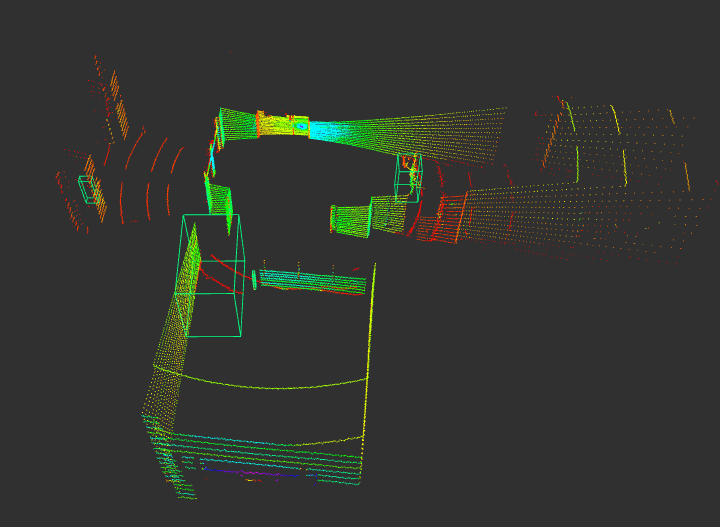
\includegraphics[width=1.0\linewidth]{figures/chap3_fig/onlineSVM/online_train_round3.png}
%     \caption{Online train round 3}
%     \label{Chap3:Fig18}
% \end{figure}

% \begin{figure}[h]
%     \centering
%     % \hspace*{-8mm}
%     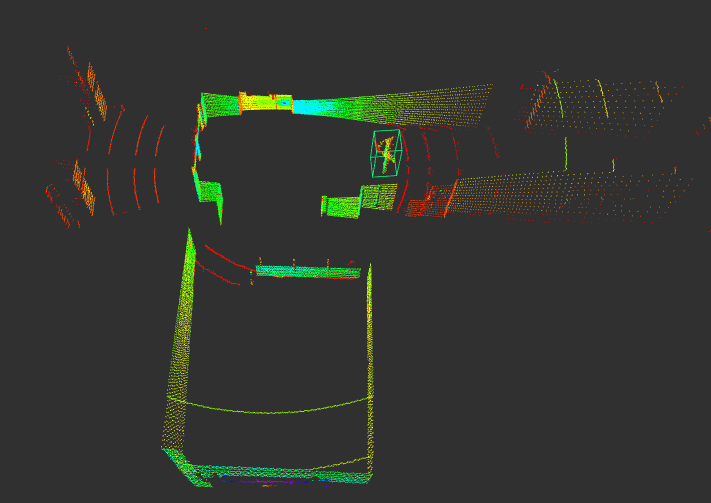
\includegraphics[width=1.0\linewidth]{figures/chap3_fig/onlineSVM/online_train_round5.png}
%     \caption{Online train round 5}
%     \label{Chap3:Fig19}
% \end{figure}

It is worth noting that the result of the online human classifier is mainly affected by the decision of 
the P-expert and N-expert of the generator in the online learning framework. As long as all assumptions and conditions such as 
human-like trajectory and static objects mentioned in section \ref{online_learning_section} are still satisfied, online human classifier
will perform effectively as in Figure \ref{Chap4:Fig23}.

%there are stacked floating elements, such as tables or figures, they will be flushed out before starting the new page.
\clearpage

%-----------------------4.2.3-----------------------------%
\subsection{Pipeline testing result}
\label{pipeline_result}

This section demonstrates the testing result of the whole pipeline whose image was shown in section \ref{whole_pipeline_intro}.

\begin{figure}[!htb]
    \centering
    % \hspace*{-8mm}
    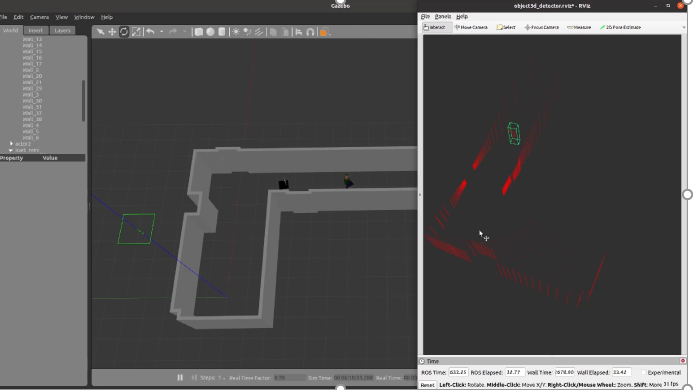
\includegraphics[scale=0.8]{figures/chap4_fig/Results/Gazebo/gazebo_simulation_result.png}
    \caption{Pipeline testing in Gazebo environment}
    \label{Chap4:fig22}
\end{figure}


\begin{figure}[!htb]
    \centering
    % \hspace*{-8mm}
    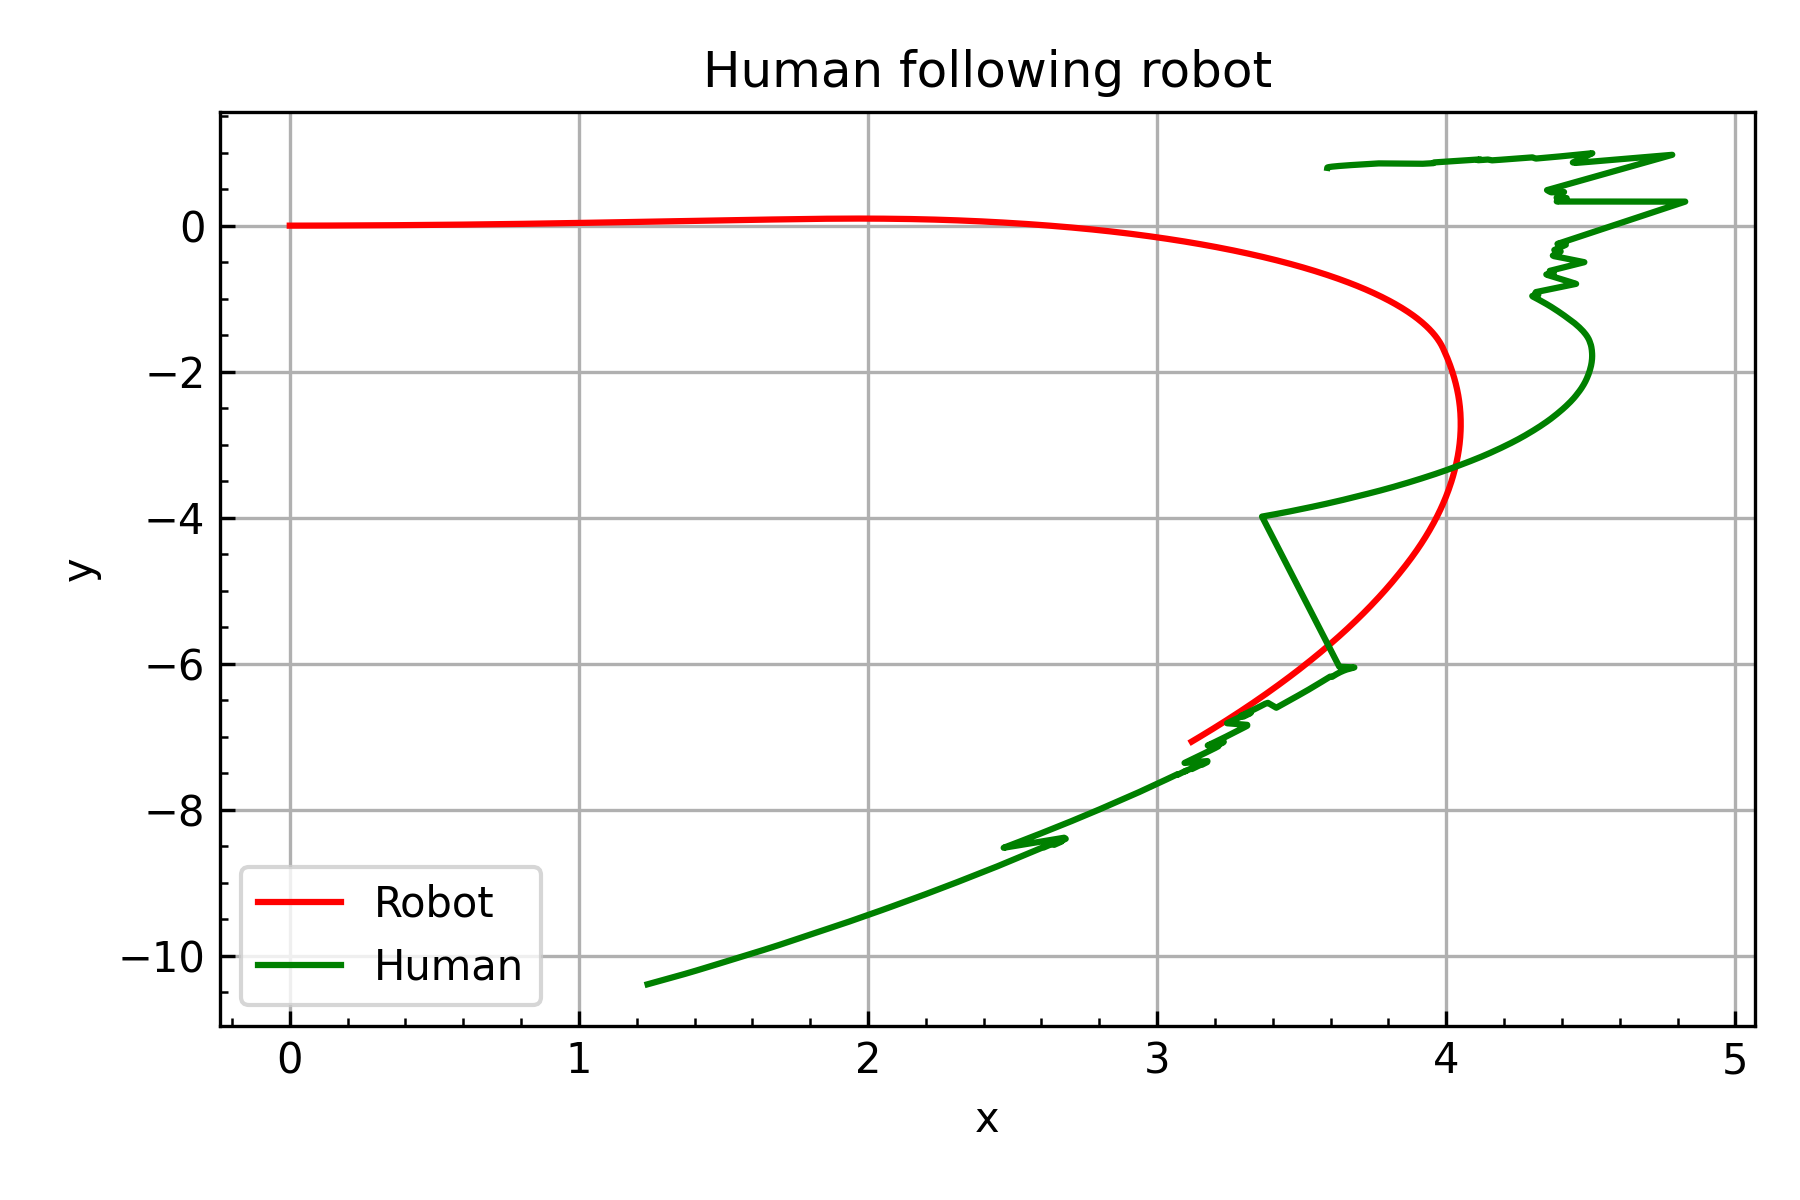
\includegraphics[scale=0.8]{figures/chap4_fig/Results/human_following_robot_gazebo_4.png}
    \caption{HFR 2D path in Gazebo simulated environment}
    \label{Chap4:Fig7}
\end{figure}

\begin{figure}[!htb]
    \centering
    \begin{subfigure}{.5\linewidth}
        \centering
        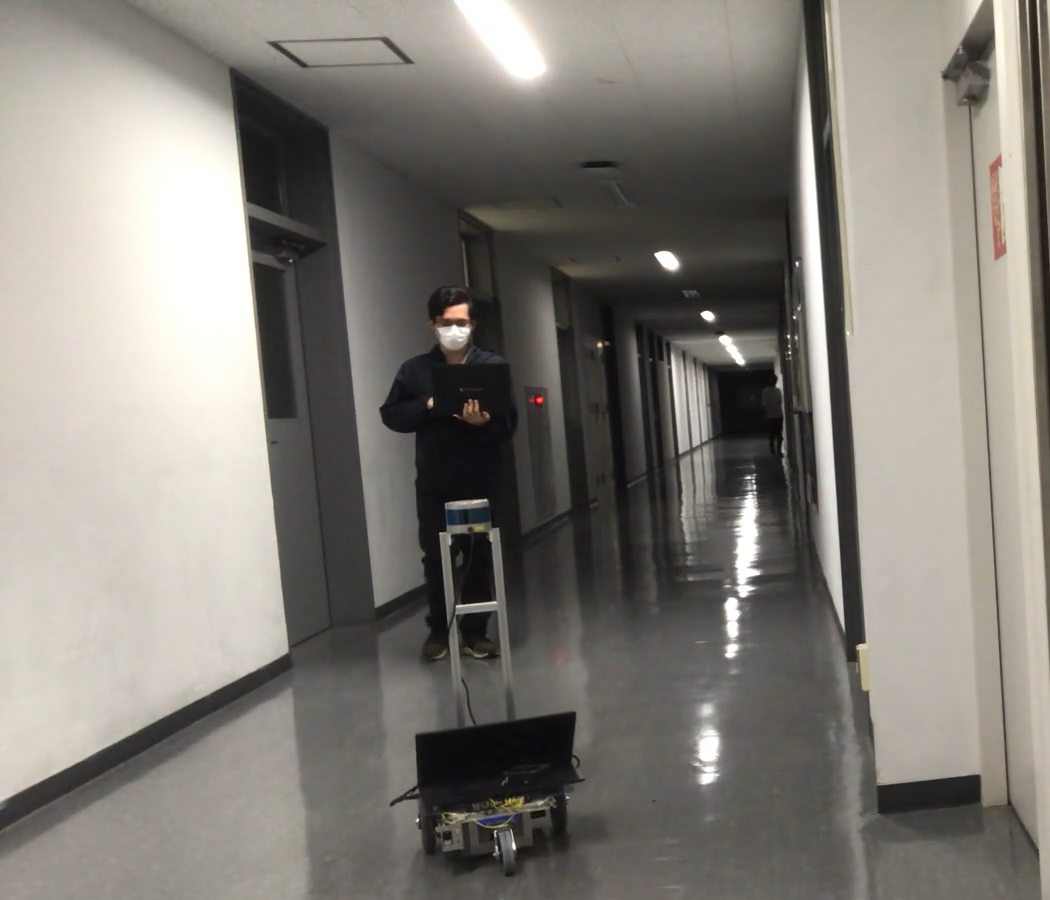
\includegraphics[width=0.9\linewidth,height = 1.0\linewidth]{figures/chap4_fig/Results/Corridor/real_corridor.png}
          \caption{HFR in real corridor}
        \label{chap4:fig20:sub1}
    \end{subfigure}%
    \begin{subfigure}{.5\linewidth}
        \centering
        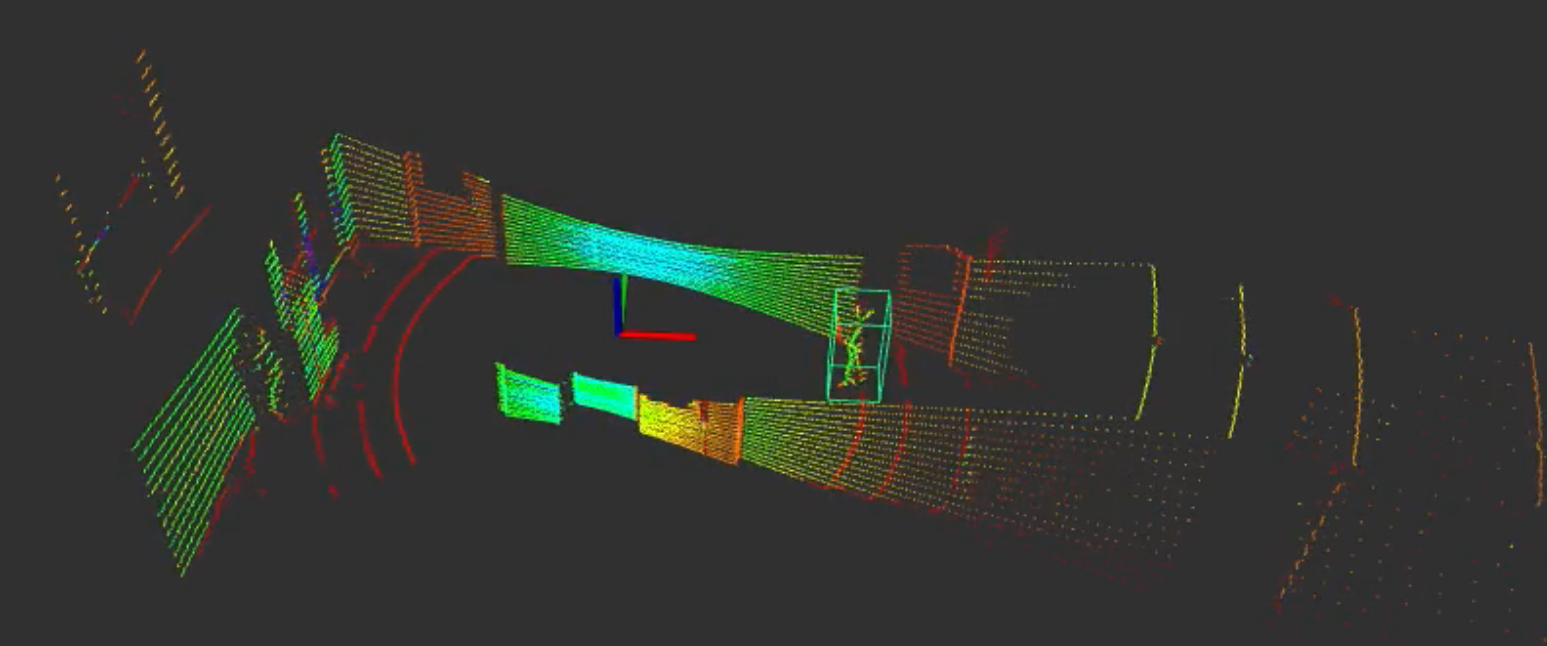
\includegraphics[width=1.0\linewidth,height = 1.0\linewidth]{figures/chap4_fig/Results/Corridor/rviz_corridor.png}
          \caption{Corresponding time in Rviz}
        \label{Chap4:fig20:sub2}
    \end{subfigure}
    \caption{Pipeline testing in corridor environment}
    \label{Chap4:fig20}
\end{figure}

\begin{figure}[!htb]
    \centering
    \hspace*{-2cm}
    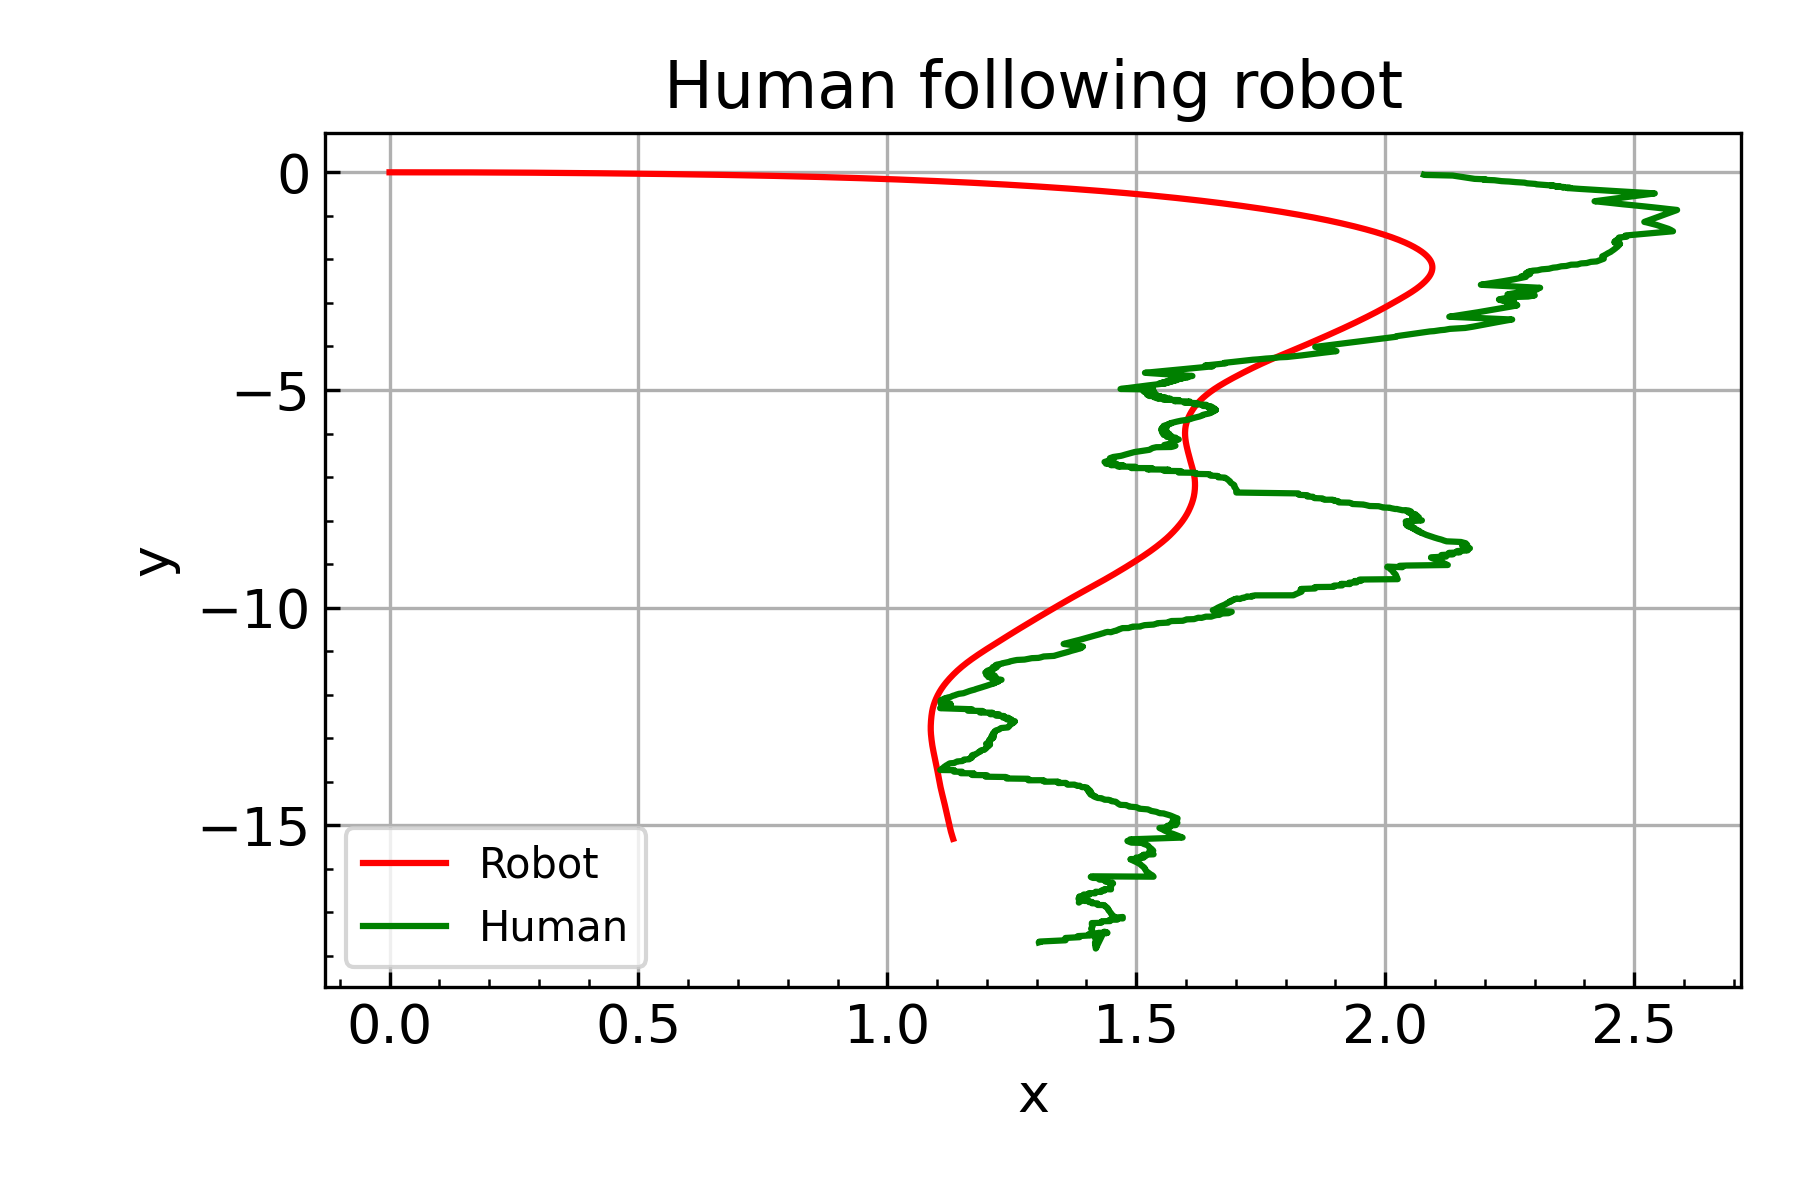
\includegraphics[scale=0.8]{figures/chap4_fig/Results/human_following_robot_corridor_5.png}
    \caption{2D path in Nagoya University Engineering Building 2 4th floor corridor}
    \label{Chap4:Fig8}
\end{figure}


\begin{figure}[!htb]
    \centering
    \begin{subfigure}{.5\linewidth}
        \centering
        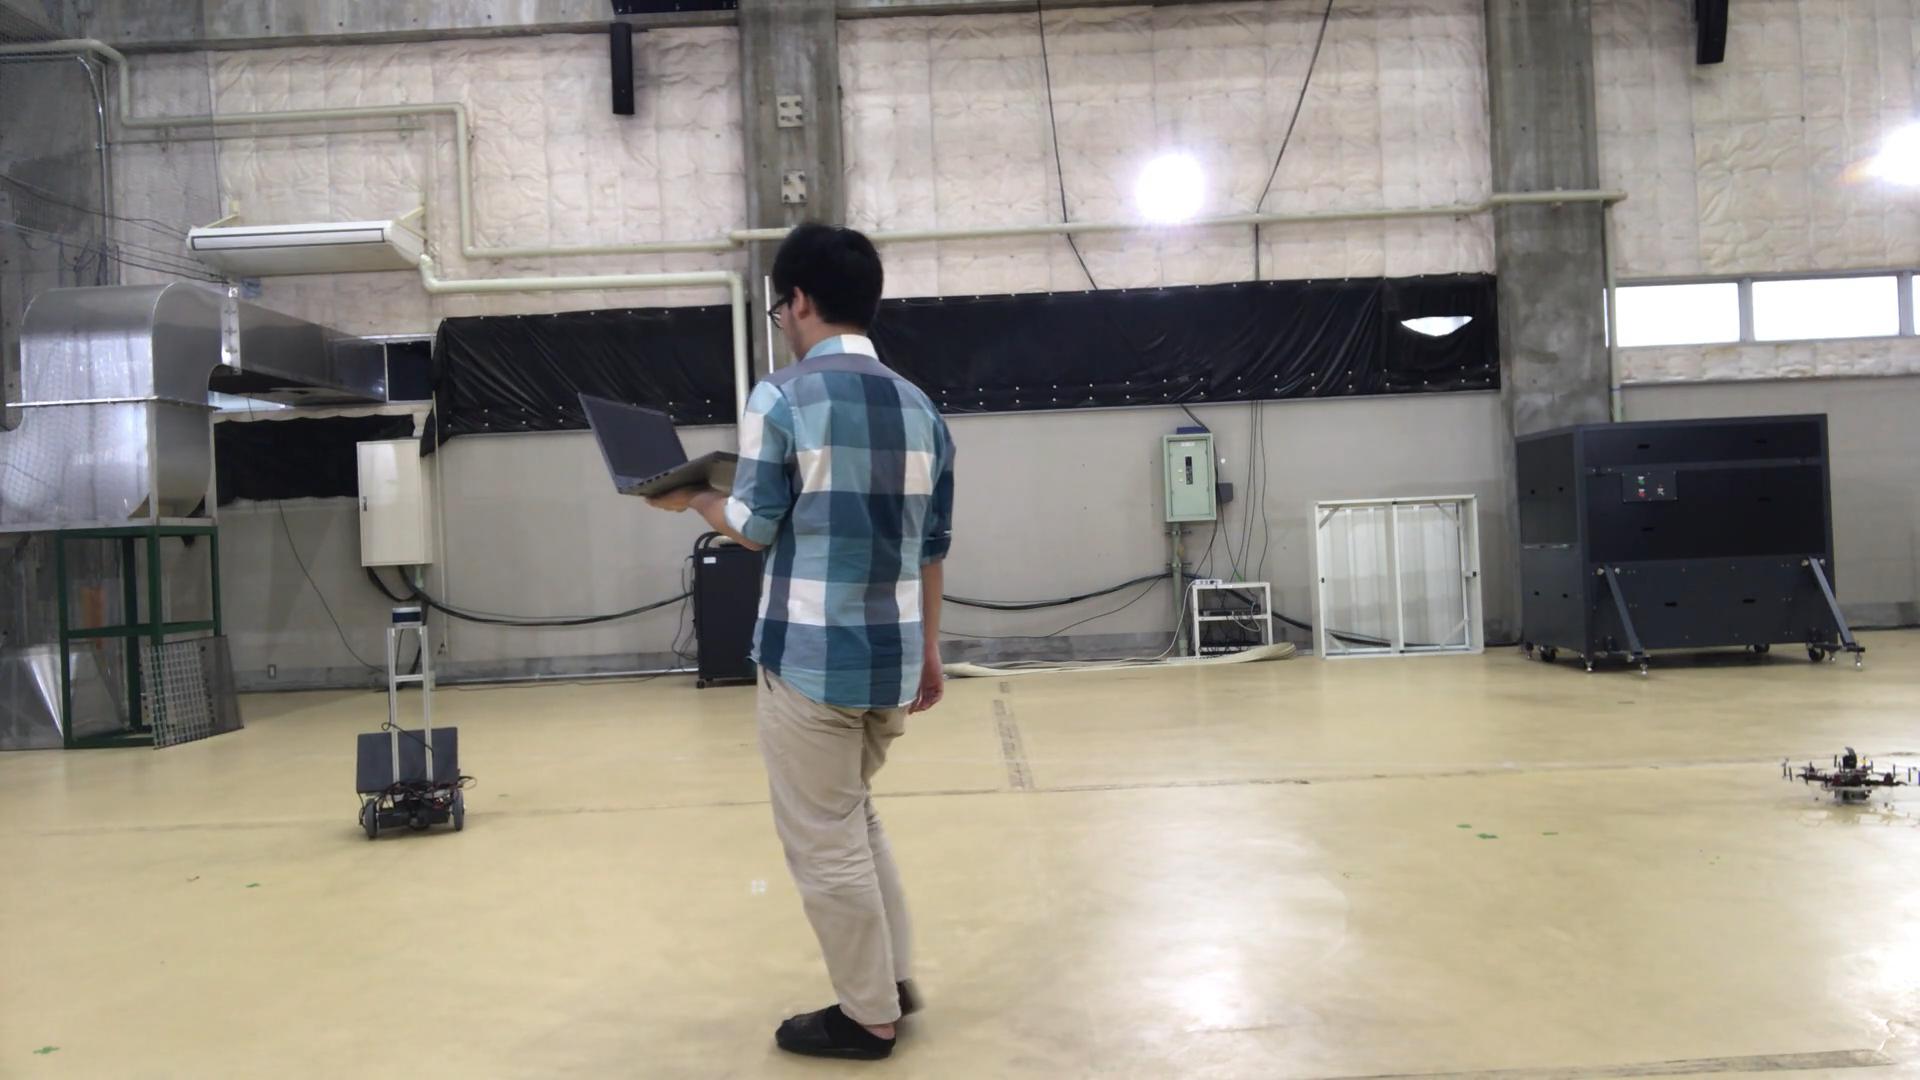
\includegraphics[width=0.95\linewidth,height = 0.5\linewidth]{figures/chap4_fig/Results/Hall/real_hall.png}
          \caption{HFR in Testing hall}
        \label{chap4:fig21:sub1}
    \end{subfigure}%
    \begin{subfigure}{.5\linewidth}
        \centering
        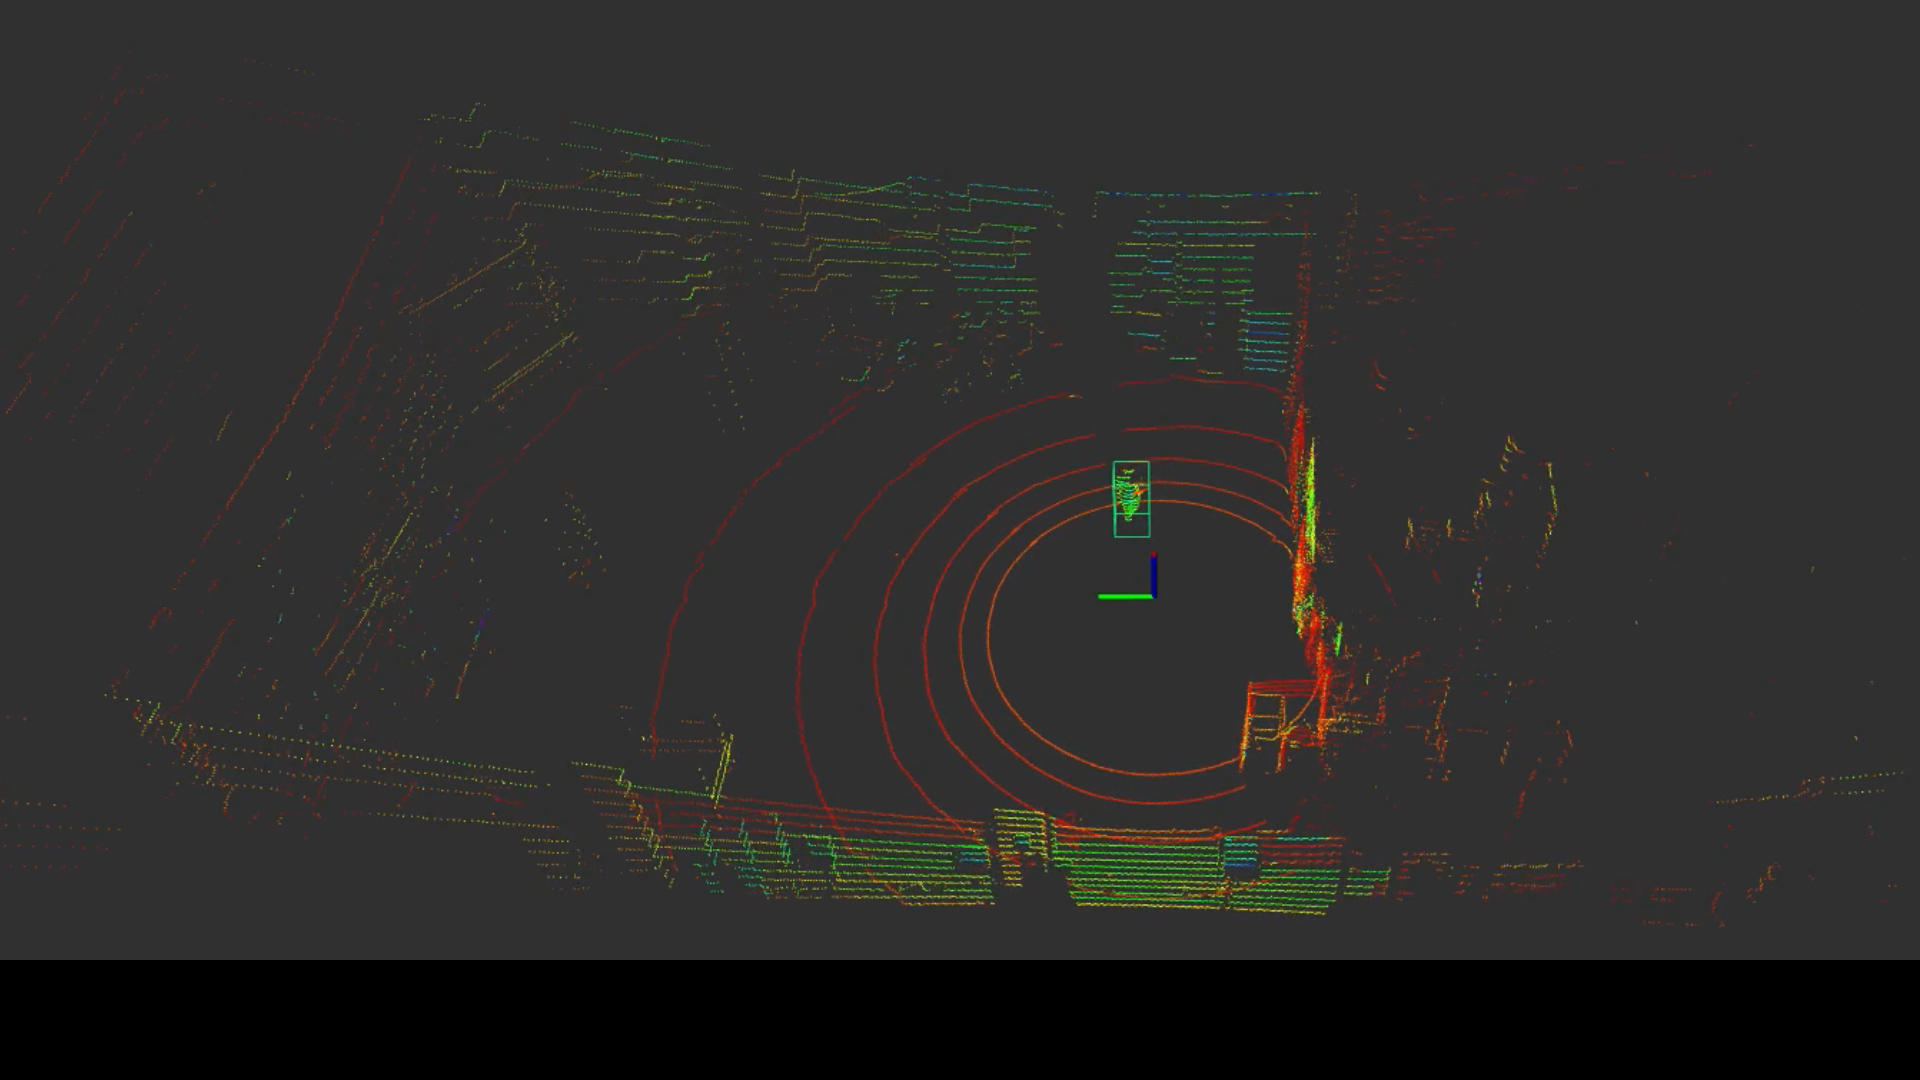
\includegraphics[width=0.95\linewidth,height = 0.5\linewidth]{figures/chap4_fig/Results/Hall/rviz_hall.png}
          \caption{Corresponding time in Rviz}
        \label{Chap4:fig21:sub2}
    \end{subfigure}
    \caption{Pipeline Test in aerospace hall environment}
    \label{Chap4:fig21}
\end{figure}


\begin{figure}[!htb]
    \centering
    % \hspace*{-8mm}
    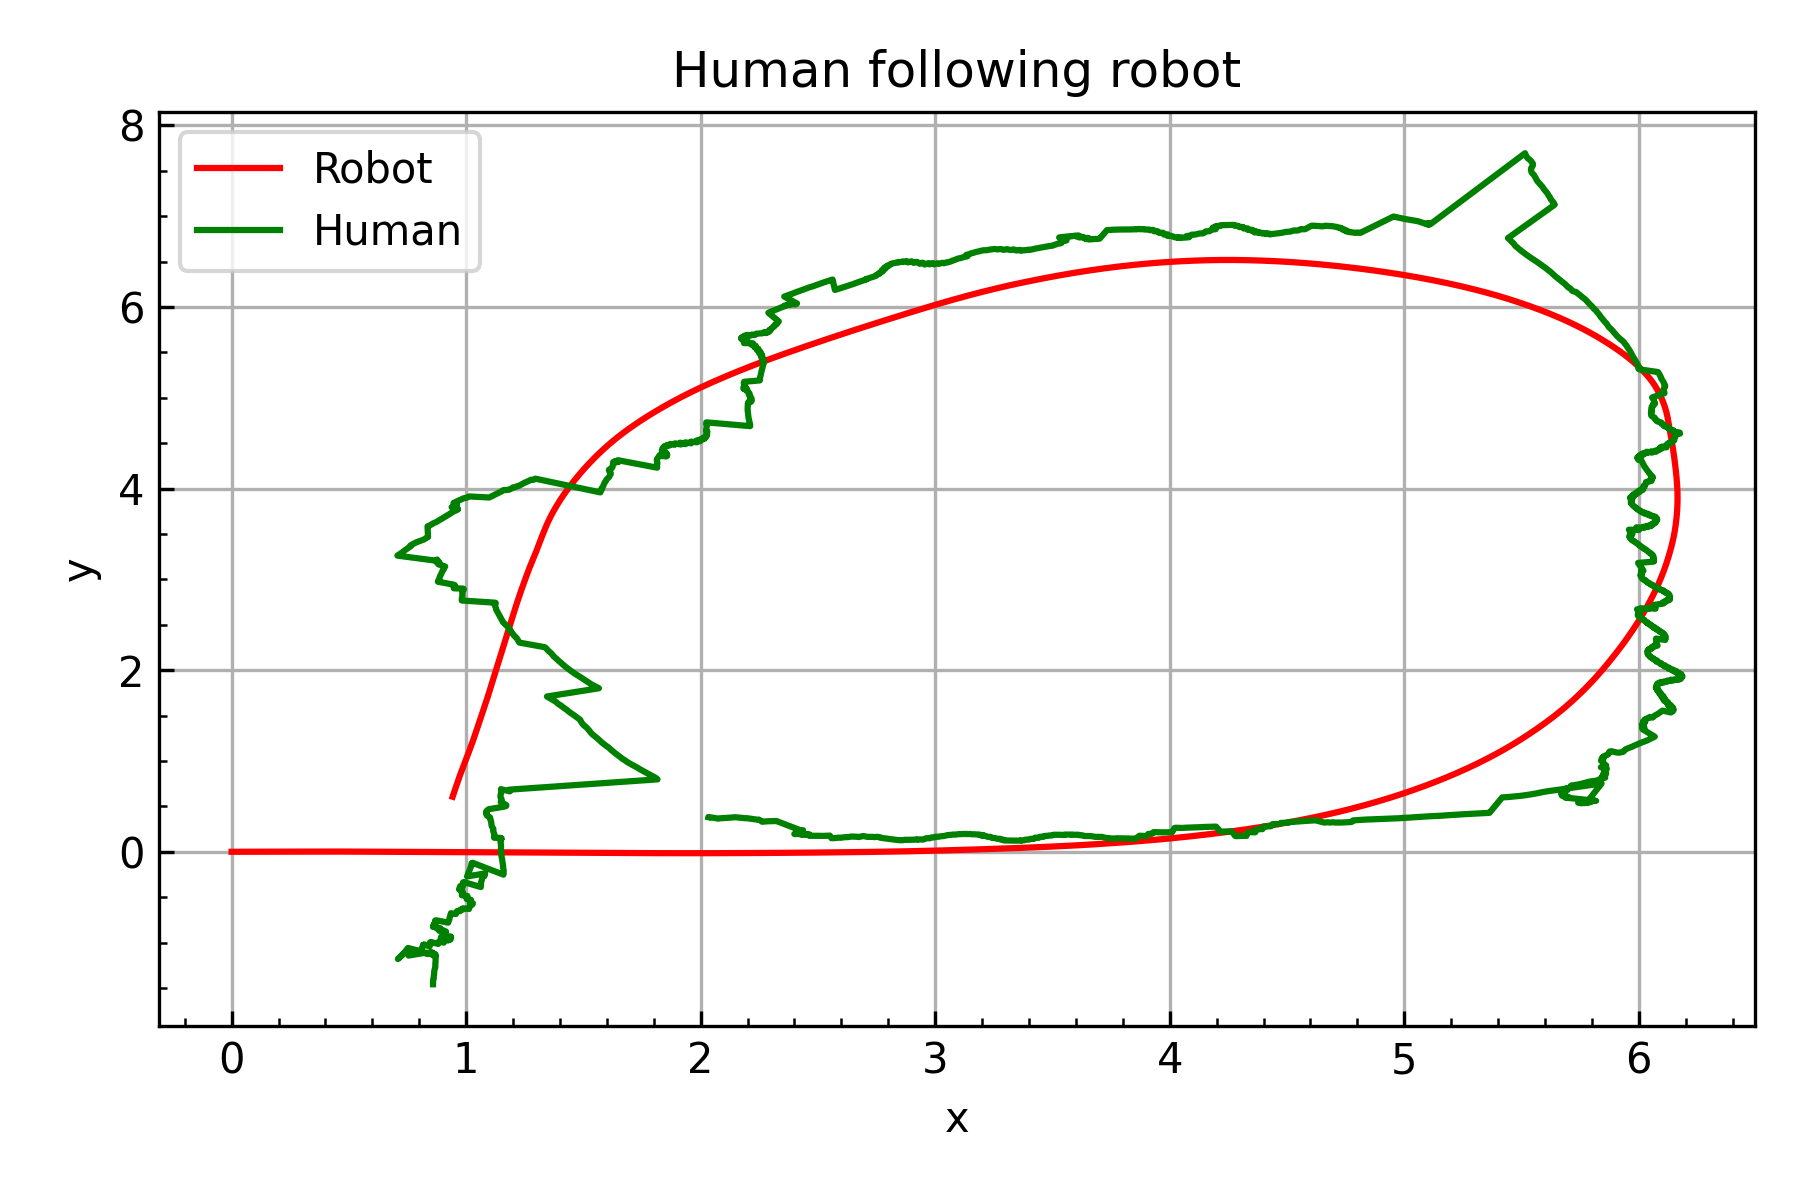
\includegraphics[scale=0.8]{figures/chap4_fig/Results/human_following_robot_hall_6.png}
    \caption{2D Path in Nagoya University ‘s Aerospace Testing hall}
    \label{Chap4:Fig9}
\end{figure}

% \begin{figure}
%     \begin{subfigure}{.5\linewidth}
%         \centering
%         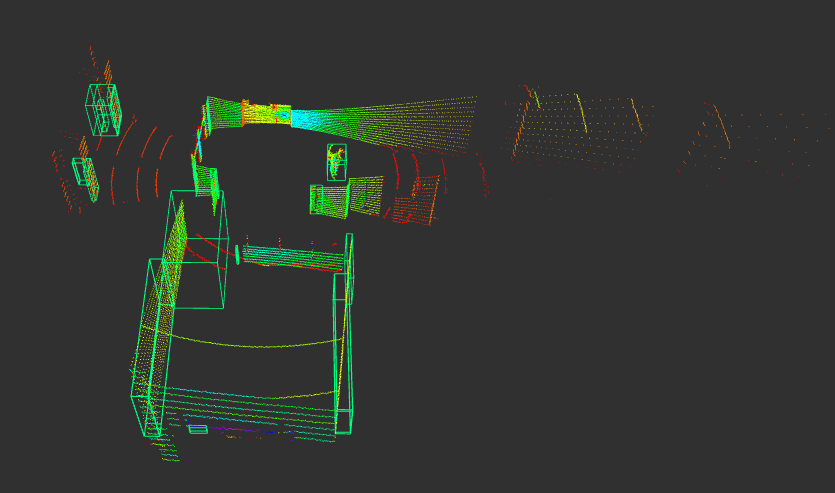
\includegraphics{figures/chap3_fig/onlineSVM/online_train_round1.png}
%         \caption{a}
%         \label{chap10:fig4:sub1}
%     \end{subfigure}%
%     \begin{subfigure}{.5\linewidth}
%         \centering
%         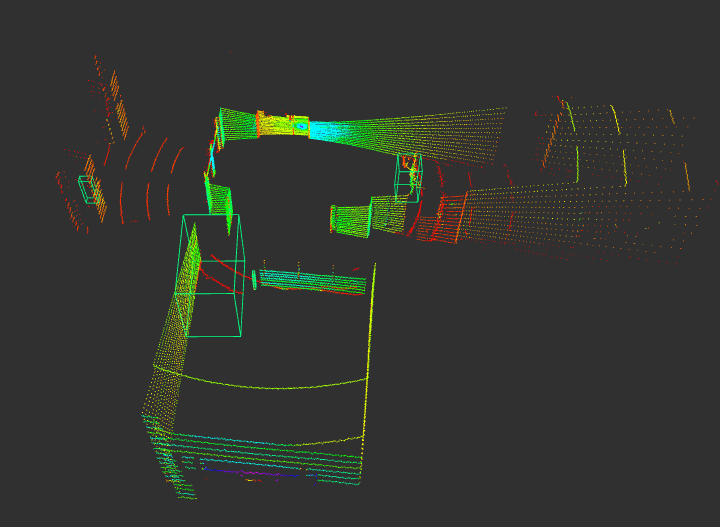
\includegraphics{figures/chap3_fig/onlineSVM/online_train_round3.png}
%         \caption{}
%         \label{chap10:fig4:sub2}
%     \end{subfigure}\\[1ex]
%     \begin{subfigure}{\linewidth}
%         \centering
%         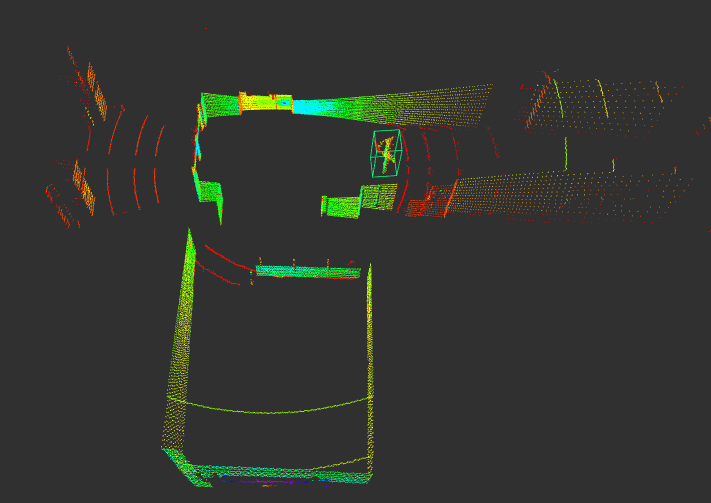
\includegraphics{figures/chap3_fig/onlineSVM/online_train_round5.png}
%         \caption{}
%         \label{chap10:fig4:sub3}
%         \end{subfigure}
%     \caption{Experiment setup}
%     \label{chap10:fig4}
% \end{figure}
\clearpage

Figure \ref{Chap4:fig22} and \ref{Chap4:Fig7} show the pipeline testing result in 
the Gazebo simulated environment. Figure \ref{Chap4:fig20} and Figure 
\ref{Chap4:Fig8} illustrate the result in the corridor while Figure \ref{Chap4:fig21} and Figure \ref{Chap4:Fig9} show the result 
in the testing hall respectively. In particular, each pair of these Figures first provides the following result in each environment with its corresponding time in Rviz (ROS Visualiation) in the first figure 
and manifests the path of both robot and human in the 2D plane in the second figure. Rviz image describes the human detection part of the pipeline by surrounding human body 
with a green box in each frame. The 2D plot describes the tracking and following part of the pipeline with green path for human and red path for robot.
In Gazebo simulation case, the robot can detect the simulated walking human and follow human's trajectory in the simulated corridor. In this simulation, we only made the human 
walk in a straight path then turn right at the corner and then go straight again. The robot follows him and creates a red curve as in Figure \ref{Chap4:Fig7}. We can observe that
the detection is not good in the simulated case with many lost target moments expressed by a green large zigzag and squiggly line. This is because the LiDAR's intensity simlation in Gazebo is not similar as in 
real life and in SVM classification, it requires 27 dimensions of LiDAR reflection intensity (see Table \ref{Chap3:Table1}) to train the human model. In fact, simulating LiDAR intensity is still complicated and demands more research work in the future.
However, despite that, the inaccuracy of human detection algorithm in the simulated case does not affect the following process because in the PID step we have added the human based velocity filter so that even the robot losts human target or misclassifies human in 
some frames, the robot can still re-find human in next frame and follow human smoothly. This happens in both other cases, in the corridor and in the testing hall. In the 
case of the corridor, the human even tried to change the direction of movement continuously, from left to right then from right to left and so on. The robot followed him smoothly and 
generated a red curve that is almost identical in shape to the human's green trajectory, as indicated in Figure \ref{Chap4:Fig8}. 
In the hall case, the robot even detected and followed the human and made a close loop path as in Figure \ref{Chap4:Fig9}. This confirms that the pipeline works well in both corridor case and testing hall case. 
The robot can still find the person even when the robot misclassifies other objects during the following process. We also notice that the robot's route is a red smooth curve while human's path is a rough green curve in all 3 cases. 
The reason for that is because the robot's path is directly calculated by its wheel encoder whereas evaluating human's position in each frame took time to operate and transfer to the global coordinate. In all 3 test cases, we make the assumption that 
there are not any obstacles that can prevent the robot from following human. This is a drawback of this pipeline and will be discussed in Chapter \ref{Chap:Conclusion_FutureWork}.